% This contents of this file will be inserted into the _Solutions version of the
% output tex document.  Here's an example:

% If assignment with subquestion (1.a) requires a written response, you will
% find the following flag within this document: <SCPD_SUBMISSION_TAG>_1a
% In this example, you would insert the LaTeX for your solution to (1.a) between
% the <SCPD_SUBMISSION_TAG>_1a flags.  If you also constrain your answer between the
% START_CODE_HERE and END_CODE_HERE flags, your LaTeX will be styled as a
% solution within the final document.

% Please do not use the '<SCPD_SUBMISSION_TAG>' character anywhere within your code.  As expected,
% that will confuse the regular expressions we use to identify your solution.
\def\assignmentnum{4 }
\def\assignmenttitle{XCS330 Problem Set \assignmentnum}

\documentclass{article}
\usepackage[top = 1.0in]{geometry}

\usepackage{graphicx}

\usepackage[utf8]{inputenc}
\usepackage{listings}
\usepackage[dvipsnames]{xcolor}
\usepackage{bm}
\usepackage{algorithm}
\usepackage{algpseudocode}
\usepackage{framed}

\definecolor{codegreen}{rgb}{0,0.6,0}
\definecolor{codegray}{rgb}{0.5,0.5,0.5}
\definecolor{codepurple}{rgb}{0.58,0,0.82}
\definecolor{backcolour}{rgb}{0.95,0.95,0.92}

\lstdefinestyle{mystyle}{
    backgroundcolor=\color{backcolour},   
    commentstyle=\color{codegreen},
    keywordstyle=\color{magenta},
    stringstyle=\color{codepurple},
    basicstyle=\ttfamily\footnotesize,
    breakatwhitespace=false,         
    breaklines=true,                 
    captionpos=b,                    
    keepspaces=true,                 
    numbersep=5pt,                  
    showspaces=false,                
    showstringspaces=false,
    showtabs=false,                  
    tabsize=2
}

\lstset{style=mystyle}

\newcommand{\di}{{d}}
\newcommand{\nexp}{{n}}
\newcommand{\nf}{{p}}
\newcommand{\vcd}{{\textbf{D}}}
\newcommand{\Int}{\mathbb{Z}}
\newcommand\bb{\ensuremath{\mathbf{b}}}
\newcommand\bs{\ensuremath{\mathbf{s}}}
\newcommand\bp{\ensuremath{\mathbf{p}}}
\newcommand{\relu} { \operatorname{ReLU} }
\newcommand{\smx} { \operatorname{softmax} }
\newcommand\bx{\ensuremath{\mathbf{x}}}
\newcommand\bh{\ensuremath{\mathbf{h}}}
\newcommand\bc{\ensuremath{\mathbf{c}}}
\newcommand\bW{\ensuremath{\mathbf{W}}}
\newcommand\by{\ensuremath{\mathbf{y}}}
\newcommand\bo{\ensuremath{\mathbf{o}}}
\newcommand\be{\ensuremath{\mathbf{e}}}
\newcommand\ba{\ensuremath{\mathbf{a}}}
\newcommand\bu{\ensuremath{\mathbf{u}}}
\newcommand\bv{\ensuremath{\mathbf{v}}}
\newcommand\bP{\ensuremath{\mathbf{P}}}
\newcommand\bg{\ensuremath{\mathbf{g}}}
\newcommand\bX{\ensuremath{\mathbf{X}}}
% real numbers R symbol
\newcommand{\Real}{\mathbb{R}}

% encoder hidden
\newcommand{\henc}{\bh^{\text{enc}}}
\newcommand{\hencfw}[1]{\overrightarrow{\henc_{#1}}}
\newcommand{\hencbw}[1]{\overleftarrow{\henc_{#1}}}

% encoder cell
\newcommand{\cenc}{\bc^{\text{enc}}}
\newcommand{\cencfw}[1]{\overrightarrow{\cenc_{#1}}}
\newcommand{\cencbw}[1]{\overleftarrow{\cenc_{#1}}}

% decoder hidden
\newcommand{\hdec}{\bh^{\text{dec}}}

% decoder cell
\newcommand{\cdec}{\bc^{\text{dec}}}

\usepackage[hyperfootnotes=false]{hyperref}
\hypersetup{
  colorlinks=true,
  linkcolor = blue,
  urlcolor  = blue,
  citecolor = blue,
  anchorcolor = blue,
  pdfborderstyle={/S/U/W 1}
}
\usepackage{nccmath}
\usepackage{mathtools}
\usepackage{graphicx,caption}
\usepackage[shortlabels]{enumitem}
\usepackage{epstopdf,subcaption}
\usepackage{psfrag}
\usepackage{amsmath,amssymb,epsf}
\usepackage{verbatim}
\usepackage{cancel}
\usepackage{color,soul}
\usepackage{bbm}
\usepackage{listings}
\usepackage{setspace}
\usepackage{float}
\definecolor{Code}{rgb}{0,0,0}
\definecolor{Decorators}{rgb}{0.5,0.5,0.5}
\definecolor{Numbers}{rgb}{0.5,0,0}
\definecolor{MatchingBrackets}{rgb}{0.25,0.5,0.5}
\definecolor{Keywords}{rgb}{0,0,1}
\definecolor{self}{rgb}{0,0,0}
\definecolor{Strings}{rgb}{0,0.63,0}
\definecolor{Comments}{rgb}{0,0.63,1}
\definecolor{Backquotes}{rgb}{0,0,0}
\definecolor{Classname}{rgb}{0,0,0}
\definecolor{FunctionName}{rgb}{0,0,0}
\definecolor{Operators}{rgb}{0,0,0}
\definecolor{Background}{rgb}{0.98,0.98,0.98}
\lstdefinelanguage{Python}{
    numbers=left,
    numberstyle=\footnotesize,
    numbersep=1em,
    xleftmargin=1em,
    framextopmargin=2em,
    framexbottommargin=2em,
    showspaces=false,
    showtabs=false,
    showstringspaces=false,
    frame=l,
    tabsize=4,
    % Basic
    basicstyle=\ttfamily\footnotesize\setstretch{1},
    backgroundcolor=\color{Background},
    % Comments
    commentstyle=\color{Comments}\slshape,
    % Strings
    stringstyle=\color{Strings},
    morecomment=[s][\color{Strings}]{"""}{"""},
    morecomment=[s][\color{Strings}]{'''}{'''},
    % keywords
    morekeywords={import,from,class,def,for,while,if,is,in,elif,else,not,and,or
    ,print,break,continue,return,True,False,None,access,as,,del,except,exec
    ,finally,global,import,lambda,pass,print,raise,try,assert},
    keywordstyle={\color{Keywords}\bfseries},
    % additional keywords
    morekeywords={[2]@invariant},
    keywordstyle={[2]\color{Decorators}\slshape},
    emph={self},
    emphstyle={\color{self}\slshape},
%
}
\lstMakeShortInline|

\pagestyle{empty} \addtolength{\textwidth}{1.0in}
\addtolength{\textheight}{0.5in}
\addtolength{\oddsidemargin}{-0.5in}
\addtolength{\evensidemargin}{-0.5in}
\newcommand{\ruleskip}{\bigskip\hrule\bigskip}
\newcommand{\nodify}[1]{{\sc #1}}
\newenvironment{answer}{\sf \begingroup\color{ForestGreen}}{\endgroup}%

\setlist[itemize]{itemsep=2pt, topsep=0pt}
\setlist[enumerate]{itemsep=6pt, topsep=0pt}

\setlength{\parindent}{0pt}
\setlength{\parskip}{4pt}
\setlist[enumerate]{parsep=4pt}
\setlength{\unitlength}{1cm}

\renewcommand{\Re}{{\mathbb R}}
\newcommand{\R}{\mathbb{R}}
\newcommand{\what}[1]{\widehat{#1}}

\renewcommand{\comment}[1]{}
\newcommand{\mc}[1]{\mathcal{#1}}
\newcommand{\half}{\frac{1}{2}}

\DeclareMathOperator*{\argmin}{arg\,min}

\def\KL{D_{KL}}
\def\xsi{x^{(i)}}
\def\ysi{y^{(i)}}
\def\zsi{z^{(i)}}
\def\E{\mathbb{E}}
\def\calN{\mathcal{N}}
\def\calD{\mathcal{D}}
\def\slack{\url{http://xcs330-scpd.slack.com/}}
\def\zipscriptalt{\texttt{python zip\_submission.py}}
\DeclarePairedDelimiter\abs{\lvert}{\rvert}%
 
\usepackage{bbding}
\usepackage{pifont}
\usepackage{wasysym}
\usepackage{amssymb}
\usepackage{framed}
\usepackage{scrextend}

\newcommand{\alns}[1] {
	\begin{align*} #1 \end{align*}
}

\newcommand{\pd}[2] {
 \frac{\partial #1}{\partial #2}
}
\renewcommand{\Re} { \mathbb{R} }
\newcommand{\btx} { \mathbf{\tilde{x}} }
\newcommand{\bth} { \mathbf{\tilde{h}} }
\newcommand{\sigmoid} { \operatorname{\sigma} }
\newcommand{\CE} { \operatorname{CE} }
\newcommand{\byt} { \hat{\by} }
\newcommand{\yt} { \hat{y} }

\newcommand{\oft}[1]{^{(#1)}}
\newcommand{\fone}{\ensuremath{F_1}}

\newcommand{\ac}[1]{ {\color{red} \textbf{AC:} #1} }
\newcommand{\ner}[1]{\textbf{\color{blue} #1}}

\newcommand{\dataset}{\mathcal{D}}
\newcommand{\task}{\mathcal{T}}
\newcommand{\supportdata}{\mathcal{D}^\mathrm{tr}}
\newcommand{\querydata}{\mathcal{D}^\mathrm{ts}}
\newcommand{\support}[1]{{#1}^\mathrm{tr}}
\newcommand{\query}[1]{{#1}^\mathrm{ts}}
\begin{document}
\pagestyle{myheadings} \markboth{}{\assignmenttitle}

% <SCPD_SUBMISSION_TAG>_entire_submission

This handout includes space for every question that requires a written response.
Please feel free to use it to handwrite your solutions (legibly, please).  If
you choose to typeset your solutions, the |README.md| for this assignment includes
instructions to regenerate this handout with your typeset \LaTeX{} solutions.
\ruleskip

\LARGE
1.b (ii)
\normalsize

% <SCPD_SUBMISSION_TAG>_1_bii
\begin{answer}
    The accuracy is very poor $(<40\%)$ for both of these models, with bert-med performing slightly better than bert-tiny. Couple of reasons

    \begin{itemize}
        \item The number of parameters in bert-tiny and bert-med is ~4.4 million and 41.7 million, respectively - which is relatively very less
        \item Just a handful of examples $(1, 2, 128)$ is being used used to fine tune the entire set of parameters 
    \end{itemize}

    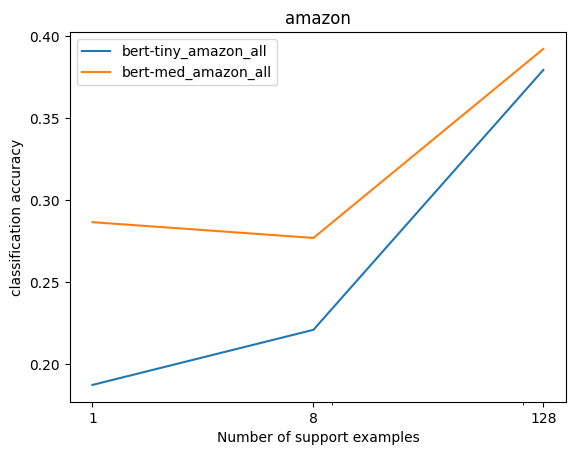
\includegraphics[width=9cm]{figures/bert_ft_all_plot.png}
    
\end{answer}
% <SCPD_SUBMISSION_TAG>_1_bii

\LARGE
1.c
\normalsize

% <SCPD_SUBMISSION_TAG>_1_c
\begin{answer}
    \begin{itemize}
        \item Number of parameters in Bert-mini = 11.2 million
        \item Space to store each parameter = 4 Byte floats
    \end{itemize}

    $\Rightarrow$ Total Disk space required to store the fine tuned model = 11.2 million $\times$ 4 bytes = $44.8 \times 10^{6}~\text{bytes} = 44.8~MB$
    
\end{answer}
% <SCPD_SUBMISSION_TAG>_1_c

\LARGE
1.d
\normalsize

% <SCPD_SUBMISSION_TAG>_1_d
\begin{answer}
    \begin{itemize}
    \item Number of parameters in Google PaLM LLM = 540 billion = $5.4 \times 10^{9}$
    \end{itemize}

    $\Rightarrow$ Disk space required to store a PaLM fine tuned model = $5.4 \times 10^{9} \times 4~\text{bytes} = 21.6~GB$
    
\end{answer}
% <SCPD_SUBMISSION_TAG>_1_d

\clearpage

\LARGE
2.b (ii)
\normalsize

% <SCPD_SUBMISSION_TAG>_2_bii
\begin{answer}
    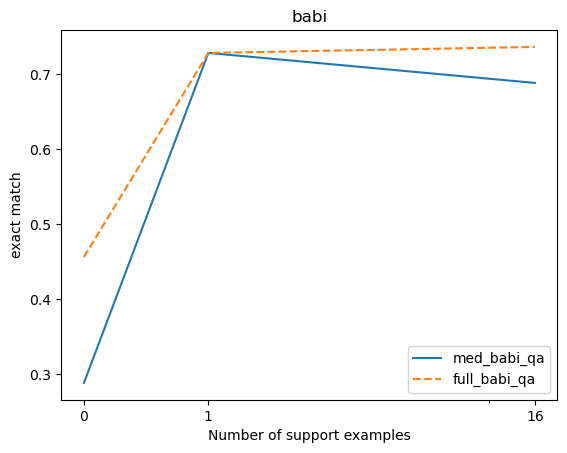
\includegraphics[width=9cm]{figures/icl_babi_plot.png}
    
    For the BABI dataset, 'qa' prompt is used which inserts ' In the ' in between every question and answer
    
    Observations
    \begin{itemize}
    \item Larger model results in better performance (accuracy). Accuracy with full sized GPT2 model (with 1.5B parameters) at $k=16$ shot = 0.736, while the accuracy with med sized GPT2 model (355M parameters) at $k=16$ is 0.688
    \item Accuracy generally increases with increasing $k$ (number of examples used in the prompt) for both medium and full sized GPT2 model. 
    \end{itemize}
    
\end{answer}
% <SCPD_SUBMISSION_TAG>_2_bii

\clearpage

\LARGE
2.c (ii)
\normalsize

% <SCPD_SUBMISSION_TAG>_2_cii
\begin{answer}
    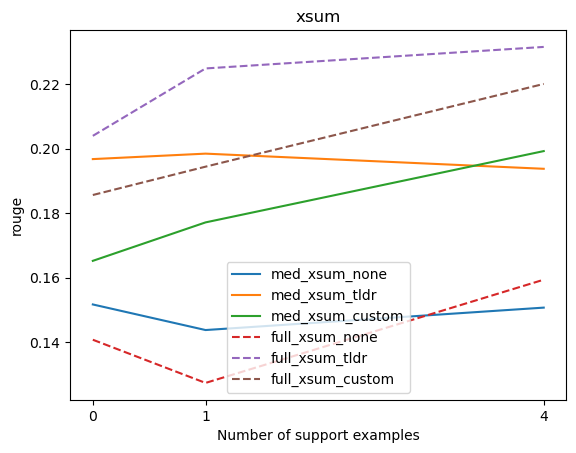
\includegraphics[width=9cm]{figures/icl_xsum_plot.png}

    Observations
    \begin{itemize}
        \item \textbf{TL;DR: } prompt outperforms no formatting with a better rogue score. Since xsum dataset measures the performance of summaries, inserting a TL;DR: prompt would help the GPT2 model with a context on what needs to be done.
        \item Custom prompt: \textbf{Summarize in one sentence: }. Since the xsum dataset consists of labels which are summaries in a single sentence, this prompt was chosen. While the custom prompt yields a better rouge score than none prompt, it has a marginally lower score when compared to the TL;DR: prompt
        \item Generally, the performance improves with larger number of support examples, i.e., rouge score for zero-shot $<$ one-shot $<$ few-shot. However, there are couple of outliers in the above plot, e.g., a) TL;DR: prompt med model: 4-shot rogue score $<$ 1-shot rogue score b) none prompt (both med and full model): 1-shot rogue score $<$ zero-shot rogue score. These are probably due to smaller sized test set 
    \end{itemize}
    
\end{answer}
% <SCPD_SUBMISSION_TAG>_2_cii

\clearpage

\LARGE
3.b
\normalsize

% <SCPD_SUBMISSION_TAG>_3_b
\begin{answer}
    \begin{itemize}
    \item Number of layers = $L$
    \item Number of parameters in the weight matrix $W_0^l$ for each layer = $d_1 \times d_2$
    \item LoRA constrained fine-tuned parameter matrix = $AB^T$
    \item Size of matrix $A$ = $d_1 \times p$
    \item Size of matrix $B$ = $d_2 \times p$
    \item Total number of parameters that would be fined-tuned using LoRA = $d_1 \times p + d_2 \times p = p(d_1+d_2)$
    \end{itemize}

    $\Rightarrow$ Ratio of the parameters fine-tuned by LoRA to the number of parameters in $W^0_l$ = $ \frac{p(d_1+d_2)}{d_1 \times d_2}$
    
    $\Rightarrow$ LoRA will provide the greatest savings in the newly-created parameters if $p << d_1, d_2$ 
    
\end{answer}
% <SCPD_SUBMISSION_TAG>_3_b

\LARGE
3.d (ii)
\normalsize

% <SCPD_SUBMISSION_TAG>_3_dii
\begin{answer}

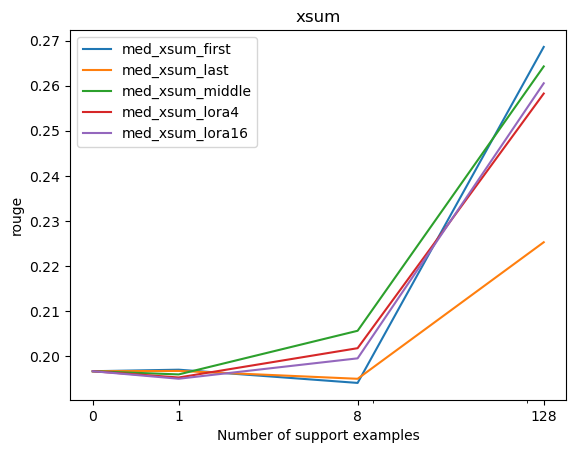
\includegraphics[width=8.5cm]{figures/lora_ft_xsum_plot.png}
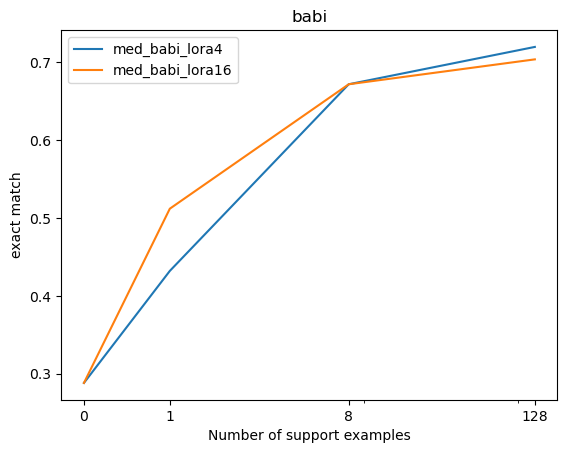
\includegraphics[width=8.5cm]{figures/lora_ft_babi_plot.png}

    Observations
    \begin{itemize}
        \item Using a higher rank LoRA residual matrix results in better performance on both xsum and babi datasets (Comparing lora4 vs. lora16)
        \item LoRA outperforms the other {first, last, middle} fine-tune algorithms for larger number of support examples, though the number of parameters that are fine tuned as less
    \end{itemize}
    
\end{answer}
% <SCPD_SUBMISSION_TAG>_3_dii

\clearpage

\LARGE
4.a
\normalsize

% <SCPD_SUBMISSION_TAG>_4_a
\begin{answer}

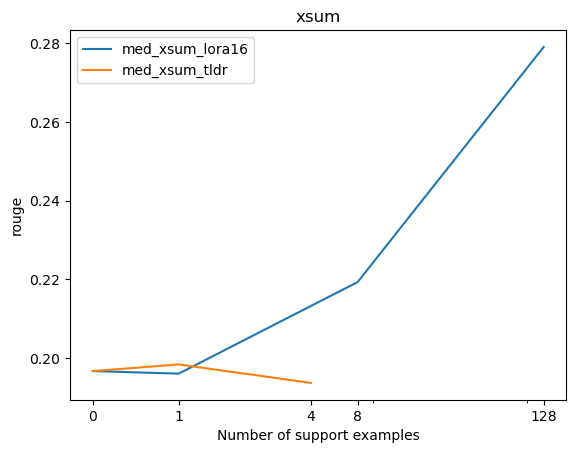
\includegraphics[width=9cm]{figures/lora_vs_icl_xsum_plot.png}

\begin{itemize}
    \item In-context learning (tldr) seems like a better choice compared to fine-tuning (lora16) when there are very little support examples $(k=0, 1)$. 
    \item With higher number of support examples $(k = 4, 8, 128)$, fine-tuning (lora16) offers better performance over in-context learning (tldr)
    \item This highlights that in-context learning doesn't learn very well from support examples - as well as fine tuning. So, whenever we have more than a couple of support examples, in-context learning wouldn't benefit from these as much as fine-tuning the model would
\end{itemize}
\end{answer}
% <SCPD_SUBMISSION_TAG>_4_a

\LARGE
4.b
\normalsize

% <SCPD_SUBMISSION_TAG>_4_b
\begin{answer}
Below table summarizes the exact match obtained for in context learning on BABI dataset for 5 random orderings of the prompt. As we can see, there is quite a deviation in these - varying from a low of 0.672 to a high of 0.728. The standard deviation for these = 0.019

In-context learning would have a higher standard deviation than fine-tuning

\begin{center}
\begin{tabular}{c c}
 \hline
 \hline
 Repeat Idx & Exact Match \\ [0.5ex] 
 \hline\hline
1 & 0.688 \\
 \hline
2 & 0.728 \\
 \hline
3 & 0.712 \\
 \hline
4 & 0.696 \\
 \hline
5 & 0.672 \\
 \hline
\end{tabular}
\end{center}

\end{answer}
% <SCPD_SUBMISSION_TAG>_4_b

\LARGE
4.c
\normalsize

% <SCPD_SUBMISSION_TAG>_4_c
\begin{answer}
    % ### START CODE HERE ###
    % ### END CODE HERE ###
\end{answer}
% <SCPD_SUBMISSION_TAG>_4_c

% <SCPD_SUBMISSION_TAG>_entire_submission

\end{document}